% Options for packages loaded elsewhere
\PassOptionsToPackage{unicode}{hyperref}
\PassOptionsToPackage{hyphens}{url}
\PassOptionsToPackage{dvipsnames,svgnames,x11names}{xcolor}
\documentclass[
  spanish,
  10pt,
  a4paper,
]{article}
\usepackage{xcolor}
\usepackage[top=22mm,bottom=22mm,left=22mm,right=22mm]{geometry}
\usepackage{amsmath,amssymb}
\setcounter{secnumdepth}{-\maxdimen} % remove section numbering
\usepackage{iftex}
\ifPDFTeX
  \usepackage[T1]{fontenc}
  \usepackage[utf8]{inputenc}
  \usepackage{textcomp} % provide euro and other symbols
\else % if luatex or xetex
  \usepackage{unicode-math} % this also loads fontspec
  \defaultfontfeatures{Scale=MatchLowercase}
  \defaultfontfeatures[\rmfamily]{Ligatures=TeX,Scale=1}
\fi
\usepackage{lmodern}
\ifPDFTeX\else
  % xetex/luatex font selection
\fi
% Use upquote if available, for straight quotes in verbatim environments
\IfFileExists{upquote.sty}{\usepackage{upquote}}{}
\IfFileExists{microtype.sty}{% use microtype if available
  \usepackage[]{microtype}
  \UseMicrotypeSet[protrusion]{basicmath} % disable protrusion for tt fonts
}{}
\usepackage{setspace}
\makeatletter
\@ifundefined{KOMAClassName}{% if non-KOMA class
  \IfFileExists{parskip.sty}{%
    \usepackage{parskip}
  }{% else
    \setlength{\parindent}{0pt}
    \setlength{\parskip}{6pt plus 2pt minus 1pt}}
}{% if KOMA class
  \KOMAoptions{parskip=half}}
\makeatother
\usepackage{longtable,booktabs,array}
\newcounter{none} % for unnumbered tables
\usepackage{calc} % for calculating minipage widths
% Correct order of tables after \paragraph or \subparagraph
\usepackage{etoolbox}
\makeatletter
\patchcmd\longtable{\par}{\if@noskipsec\mbox{}\fi\par}{}{}
\makeatother
% Allow footnotes in longtable head/foot
\IfFileExists{footnotehyper.sty}{\usepackage{footnotehyper}}{\usepackage{footnote}}
\makesavenoteenv{longtable}
\usepackage{graphicx}
\makeatletter
\newsavebox\pandoc@box
\newcommand*\pandocbounded[1]{% scales image to fit in text height/width
  \sbox\pandoc@box{#1}%
  \Gscale@div\@tempa{\textheight}{\dimexpr\ht\pandoc@box+\dp\pandoc@box\relax}%
  \Gscale@div\@tempb{\linewidth}{\wd\pandoc@box}%
  \ifdim\@tempb\p@<\@tempa\p@\let\@tempa\@tempb\fi% select the smaller of both
  \ifdim\@tempa\p@<\p@\scalebox{\@tempa}{\usebox\pandoc@box}%
  \else\usebox{\pandoc@box}%
  \fi%
}
% Set default figure placement to htbp
\def\fps@figure{htbp}
\makeatother
\ifLuaTeX
\usepackage[bidi=basic,shorthands=off]{babel}
\else
\usepackage[bidi=default,shorthands=off]{babel}
\fi
\ifLuaTeX
  \usepackage{selnolig} % disable illegal ligatures
\fi
\setlength{\emergencystretch}{3em} % prevent overfull lines
\providecommand{\tightlist}{%
  \setlength{\itemsep}{0pt}\setlength{\parskip}{0pt}}

\usepackage{amsmath,amssymb,mathtools}
\usepackage{microtype}
\usepackage{fancyhdr}
\usepackage{needspace}
\usepackage{etoolbox}
\usepackage{float}
\usepackage{caption}
\captionsetup{font=small,labelformat=empty,skip=7pt}
\floatplacement{figure}{H}
\definecolor{DocBlue}{HTML}{173F57}
\definecolor{DocGray}{HTML}{52616C}
\pagestyle{fancy}
\fancyhf{}
\fancyhead[L]{\small\sffamily\color{DocGray} pySNSPD | Desarrollo del modelo}
\fancyhead[R]{\small\sffamily\color{DocGray} Revisión 0.4}
\fancyfoot[L]{\small\sffamily\color{DocGray} 9 de septiembre de 2026}
\fancyfoot[R]{\small\sffamily\thepage}
\setlength{\headheight}{15pt}
\setlength{\emergencystretch}{2em}
\setlength{\parskip}{5pt plus 1pt}
\setlength{\parindent}{0pt}
\widowpenalty=10000
\clubpenalty=10000
\displaywidowpenalty=10000
\predisplaypenalty=10000
\renewcommand{\arraystretch}{1.16}
\AtBeginEnvironment{longtable}{\small}
\pretocmd{\section}{\Needspace{6\baselineskip}}{}{}
\pretocmd{\subsection}{\Needspace{5\baselineskip}}{}{}
\AtBeginDocument{\hypersetup{colorlinks=true,linkcolor=DocBlue,urlcolor=DocBlue}}
\allowdisplaybreaks[1]
\usepackage{bookmark}
\IfFileExists{xurl.sty}{\usepackage{xurl}}{} % add URL line breaks if available
\urlstyle{same}
\hypersetup{
  pdftitle={D. Síntesis{,} ecuaciones y verificaciones},
  pdflang={es},
  colorlinks=true,
  linkcolor={Maroon},
  filecolor={Maroon},
  citecolor={Blue},
  urlcolor={Blue},
  pdfcreator={LaTeX via pandoc}}

\title{D. Síntesis, ecuaciones y verificaciones}
\usepackage{etoolbox}
\makeatletter
\providecommand{\subtitle}[1]{% add subtitle to \maketitle
  \apptocmd{\@title}{\par {\large #1 \par}}{}{}
}
\makeatother
\subtitle{Contrato continuo del candidato experimental · Documento 4 de
5}
\author{}
\date{9 de septiembre de 2026 · Revisión 0.4}

\begin{document}
\maketitle

{
\setcounter{tocdepth}{2}
\tableofcontents
}
\setstretch{1.07}
\newpage

\section{D.0. Decisión y resultado de la
revisión}\label{d.0.-decisiuxf3n-y-resultado-de-la-revisiuxf3n}

La revisión 0.4 fija \textbf{un candidato matemático para ensayos en un
dominio de admisión restringido}, con poblaciones espectrales, una
energía común para fuerza y corriente, movilidad KWT y circuito
acoplado. No se modifica el solver de producción. Las verificaciones
independientes detectaron tres obstáculos: la fuerza de núcleo depende
fuertemente del parámetro efectivo que lo completa; ciertos estados
pierden la estabilidad de las perturbaciones espaciales cortas; y la DOS
fonónica disponible no tiene todavía unidades y normalización
admisibles. Por ello \textbf{no se recomienda promover este candidato a
producción} con los datos actuales.

Esto no invalida el avance de A--C. La fuerza microscópica ya contiene
el depareamiento por corriente; conservar además el término GL
correspondiente lo contaría dos veces. Pero corregir esa contabilidad no
basta para definir la física en un cero del condensado. La prueba de
vórtice de C distingue una energía total que cambia 1.26\% de una fuerza
máxima cuya dispersión alcanza 205\%. También detecta rigideces
espaciales distintas de la referencia linealizada de Usadel. Son
diagnósticos que anticipan cambios en un transitorio, aunque todavía no
calculen una latencia del detector.

{\def\LTcaptype{none} % do not increment counter
\begin{longtable}[]{@{}
  >{\raggedright\arraybackslash}p{(\linewidth - 4\tabcolsep) * \real{0.3333}}
  >{\raggedright\arraybackslash}p{(\linewidth - 4\tabcolsep) * \real{0.3333}}
  >{\raggedright\arraybackslash}p{(\linewidth - 4\tabcolsep) * \real{0.3333}}@{}}
\toprule\noalign{}
\begin{minipage}[b]{\linewidth}\raggedright
Bloque
\end{minipage} & \begin{minipage}[b]{\linewidth}\raggedright
Decisión que se incorpora
\end{minipage} & \begin{minipage}[b]{\linewidth}\raggedright
Sustento de 0.4
\end{minipage} \\
\midrule\noalign{}
\endhead
\bottomrule\noalign{}
\endlastfoot
Catálogo electrónico & Usadel local de acoplamiento débil, con amplitud
independiente & A: derivadas, integrabilidad y rama retardada
verificadas de nuevo \\
Poblaciones & Distribuciones electrónicas y fonónicas completas & B:
igual energía permite fuerzas diferentes por un factor 25.19 \\
Relajación electrónica & BGK que conserva energía; tiempo cinético de
entrada independiente & B: conservación y sensibilidad temporal
explícitas \\
Depósito de calor & Fuente espectral efectiva definida desde ocupación
nula & B: normalización y trayectoria desde el vacío verificadas \\
Condensado & Energía cartesiana de C con \(\delta=0.10\Delta_0\) finito
& C: primera variación, calibre y disipación verificadas; núcleo sin
validar \\
Transporte y circuito & Difusión electrónica, escape fonónico local,
continuaciones 1D y carga paralela & B/C y prueba circuital
independiente de D \\
\end{longtable}
}

La sección D.1 reúne las ecuaciones continuas que realmente definen ese
candidato. Los diagnósticos no se añaden como mecanismos físicos ni como
fuentes nuevas. Los parámetros que requieren medición o procedencia
siguen siendo entradas identificadas; no se los oculta eligiendo un
número que ajuste una traza.

\section{D.1. Sistema continuo completo para implementación
experimental}\label{d.1.-sistema-continuo-completo-para-implementaciuxf3n-experimental}

\subsection{D.1.1. Dominio, incógnitas y
convenciones}\label{d.1.1.-dominio-incuxf3gnitas-y-convenciones}

Se resuelve una película 2D \(\mathcal W\) de espesor uniforme \(d_f\),
conectada a dos continuaciones longitudinales 1D del mismo material. En
2D, \(dV=d_f\,d^2r\); en una continuación de sección \(S_c\),
\(dV=S_c\,d\ell\). Las densidades que siguen se expresan por volumen;
estas medidas se usan al integrar energías y flujos. Los extremos
remotos representan reservorios superconductores, no bordes térmicos
colocados junto al impacto. El intervalo temporal es \(t\geq t_0\),
después de la cascada inicial no resuelta.

Las incógnitas son

\[
\Delta(\mathbf r,t)\in\mathbb C,\quad p(x,\mathbf r,t),\quad
n(\Omega,\mathbf r,t),\quad \phi(\mathbf r,t),\quad I(t).
\tag{D.1}
\]

\(p\) es la ocupación de un estado de excitación electrónico, \(n\) la
ocupación de un modo fonónico, \(\phi\) el potencial eléctrico e \(I\)
la corriente de la rama del detector. \(\phi\) satisface una restricción
elíptica instantánea, no una ecuación capacitiva. La temperatura
equivalente será una función de \(p\), no otra incógnita dinámica. Se
adopta simetría electrón--hueco, aproximación difusiva y espectro local
adiabático: el catálogo se acomoda a los campos presentes mientras las
ocupaciones pueden ser no térmicas. No se resuelven aquí el
desequilibrio espectral de carga, el campo magnético propio ni el
transporte lateral fonónico.

Con \(e>0\), \(N_0\) la DOS normal por espín {[}J\(^{-1}\)m\(^{-3}\){]},
\(D\) la difusividad y \(\sigma_n=2e^2N_0D\), las convenciones son

\[
\begin{gathered}
\mathcal D_i=\partial_i-\frac{2ie}{\hbar}A_i,\qquad
D_t=\partial_t+\frac{2ie}{\hbar}\phi,\qquad
\mathbf A=0,\quad\mathbf E=-\nabla\phi,\\
\rho_\Delta=|\Delta|^2,\quad P_i=\operatorname{Im}(\Delta^*\mathcal D_i\Delta),\quad
s_\delta=\rho_\Delta+\delta^2,\\
m=\rho_\Delta/s_\delta,\qquad \mathbf q_\delta=\mathbf P/s_\delta,\qquad
\delta=0.10\Delta_0,\quad \Delta_0=\pi e^{-\gamma_E}k_BT_c,\\
\Gamma=\frac{\hbar Dq_\delta^2}{2},\qquad
K_0=\frac{\pi N_0\hbar D}{8k_BT_c}.
\end{gathered}\tag{D.2}
\]

\(\gamma_E\) es la constante de Euler. \(\rho_\Delta\) no es la DOS
\(N_1(E)\). \(\delta\) tiene unidades de energía y es un parámetro
efectivo fijo, no un corte de malla que deba tender a cero. Se escribe
el operador covariante para conservar el origen de las fuerzas; el
escenario seleccionado evalúa \(\mathbf A=0\). \textbf{Origen:} A.2 y
C.8--C.9.

\subsection{D.1.2. Catálogo espectral y energía del
fondo}\label{d.1.2.-catuxe1logo-espectral-y-energuxeda-del-fondo}

Para cada amplitud y \(\Gamma\) se resuelve la rama retardada causal

\[
\begin{gathered}
|\Delta|c^R=(\Gamma c^R-iz)s^R,\qquad (c^R)^2+(s^R)^2=1,
\qquad z=E+i0^+,\\
c^R=N_1+iR_1,\qquad s^R=N_2+iR_2,\qquad c^R\longrightarrow1
\quad(E\longrightarrow\infty).
\end{gathered}\tag{D.3}
\]

La continuación se sigue en la ecuación original; una raíz de un
polinomio obtenido al elevar al cuadrado no basta para elegir rama.
\(N_1\geq0\) cuenta estados. Las integrales se entienden en el límite
causal, con el regulador numérico verificado, no como un ensanchamiento
inelástico nuevo. En particular, los umbrales los establece el soporte
espectral, no un corte artificial en \(|\Delta|\).

La representación que se evoluciona sigue el número acumulado de
estados:

\[
x(E)=\int_0^E N_1(E')\,dE',\quad E=E(x;|\Delta|,q_\delta),
\quad p(x)=f(E(x)),\quad dx=N_1\,dE.
\tag{D.4}
\]

\(x\) tiene unidades de energía, pero etiqueta estados: \(4N_0dx\) es su
densidad de conteo con las degeneraciones adoptadas. La inversa sólo se
usa sobre el soporte con estados. Un intervalo vacío del gap no recibe
ocupaciones.

Para obtener el fondo se evalúa también el catálogo de Matsubara a una
temperatura auxiliar \(T>0\):

\[
\begin{gathered}
\epsilon_n=(2n+1)\pi k_BT,\qquad c_n=\cos\Theta_n,\quad s_n=\sin\Theta_n,\\
\epsilon_n s_n-|\Delta|c_n+\Gamma s_nc_n=0,\qquad n\geq0,\\
f_e^{\rm FD}=-\frac{\pi^2}{3}N_0(k_BT)^2+N_0|\Delta|^2\ln\frac{T}{T_c}\\
\hspace{4mm}+2\pi N_0k_BT\sum_{n\geq0}
\left[\frac{|\Delta|^2}{\epsilon_n}+2\epsilon_n(1-c_n)
-2|\Delta|s_n+\Gamma s_n^2\right].
\end{gathered}\tag{D.5}
\]

Se usa la rama espectral física a amplitud fija, sin imponer la ecuación
de gap. La suma renormalizada y su cola se convergen conjuntamente. El
término normal de D.5 fija la referencia de energía, necesaria para el
balance.

La energía del vacío emparejado queda definida por

\[
\begin{gathered}
U_{\rm vac}(|\Delta|,q_\delta)=\lim_{T\to0}f_e^{\rm FD}(T,|\Delta|,q_\delta),\\
U_{\rm vac}(|\Delta|,0)=N_0|\Delta|^2
\left[\ln\frac{|\Delta|}{\Delta_0}-\frac12\right].
\end{gathered}\tag{D.6}
\]

También puede evaluarse a cualquier \(T_a>0\) auxiliar usando la
identidad del mismo espectro ideal,

\[
U_{\rm vac}=f_e^{\rm FD}(T_a,|\Delta|,q_\delta)
+4N_0k_BT_a\int_0^\infty\ln[1+e^{-E(x)/(k_BT_a)}]dx.
\tag{D.7}
\]

La independencia respecto de \(T_a\) es un control de la tabla, no una
temperatura física adicional. D.7 procede de minimizar la energía de
ocupaciones menos su entropía; evita exigir un límite numérico mal
resuelto en \(T=0\). \textbf{Origen:} A.12, A.16, A.23 y B.43--B.48.

\subsection{D.1.3. Energía, fuerza y corriente
compartidas}\label{d.1.3.-energuxeda-fuerza-y-corriente-compartidas}

La densidad electrónica y la energía espacial que se implementan son

\[
\begin{gathered}
u_e=U_{\rm vac}+4N_0\int_0^\infty E(x)p(x)dx,\\
e_\delta=u_e+K_0\left[\sum_i|\mathcal D_i\Delta|^2-\rho_\Delta q_\delta^2\right],
\qquad\mathcal U_\delta=\int_{\mathcal V}e_\delta\,dV.
\end{gathered}\tag{D.8}
\]

Las derivadas locales a ocupaciones \(p(x)\) fijas son

\[
\begin{gathered}
X_{|\Delta|}=\partial_{|\Delta|}U_{\rm vac}
+4N_0\int_0^\infty R_2(E)f(E)dE,\\
\boldsymbol\Pi=\frac{\hbar\sigma_n}{2e^2}\mathbf q_\delta
\int_0^\infty2N_2R_2[1-2f(E)]dE.
\end{gathered}\tag{D.9}
\]

\(X_{|\Delta|}\) y \(\boldsymbol\Pi\) son derivadas del catálogo local.
La corriente de toda la película se obtiene después de variar también
\(\mathbf q_\delta\) y el término espacial, no tomando solamente
\(2e\boldsymbol\Pi/\hbar\).

\[
\begin{gathered}
\mathbf V_\delta=\frac{\boldsymbol\Pi-2K_0\rho_\Delta\mathbf q_\delta}{s_\delta},\qquad
h_\rho=\frac{X_{|\Delta|}}{2|\Delta|}-\frac{\boldsymbol\Pi\cdot\mathbf q_\delta}{s_\delta}
+K_0q_\delta^2(2m-1),\\
\mathscr F_\delta=\frac{\delta\mathcal U_\delta}{\delta\Delta^*}
=h_\rho\Delta-K_0\mathcal D_i\mathcal D_i\Delta
-i\mathbf V_\delta\cdot\boldsymbol{\mathcal D}\Delta
-\frac{i}{2}(\nabla\cdot\mathbf V_\delta)\Delta,\\
\mathbf j_{s,\delta}=\frac{2e}{\hbar}
\left[m\boldsymbol\Pi+2K_0(1-m^2)\mathbf P\right].
\end{gathered}\tag{D.10}
\]

Se suma el índice espacial \(i\). La definición primaria de la fuerza es
la primera variación cartesiana de D.8. En \(\Delta=0\) se evalúan los
productos continuos, como \([X_{|\Delta|}/|\Delta|]\Delta\to0\) cuando
\(X=O(|\Delta|\ln|\Delta|)\); no se forma un arreglo con \(h_\rho=0/0\).
Una división aislada y su posterior recorte no implementan D.8. La
evolución espacial sólo se admite mientras conserve la positividad del
símbolo principal definido en D.36; regularizar un cociente no demuestra
esa propiedad. \textbf{Origen:} B.49--B.50 y C.9--C.13.

\subsection{D.1.4. Temperatura equivalente y ley temporal del
condensado}\label{d.1.4.-temperatura-equivalente-y-ley-temporal-del-condensado}

Se calcula \(T_E\geq0\) por inversión a espectro instantáneo fijo:

\[
\begin{gathered}
f_{\rm FD}(E,T)=\frac{1}{e^{E/(k_BT)}+1},\qquad
4N_0\int_0^\infty E p\,dx
=4N_0\int_0^\infty E f_{\rm FD}(E,T_E)dx,\\
T_{\rm mob}=\max(T_E,T_b),\quad
A_0=N_0\sqrt{\frac{1+T_{\rm mob}/T_c}{2}},\qquad
\tau_0=\frac{\pi\hbar}{8k_BT_c},\\
\tau_\psi^{-1}=\frac{T_{\rm mob}/T_c}{0.50\,{\rm ps}}
+\frac{(T_{\rm mob}/T_c)^3}{2.47\,{\rm ps}},\qquad
R=\sqrt{1+4\rho_\Delta\tau_\psi^2/\hbar^2}.
\end{gathered}\tag{D.11}
\]

El valor \(T_E=0\) se entiende por continuidad. En el continuo ideal la
energía térmica crece monótonamente; en una tabla finita se debe
verificar que la energía esté dentro de su rango y ampliar el corte si
hace falta. \(T_{\rm mob}>0\) evita extrapolar a un tiempo infinito en
una celda sin excitaciones. Los tiempos de D.11 son la movilidad
efectiva heredada de C, no el tiempo cinético BGK que se introduce más
abajo.

La ecuación compleja conservada en el tiempo es

\[
\frac{A_0\tau_0}{R}
\left[D_t\Delta+\frac{2\tau_\psi^2}{\hbar^2}
\partial_t\rho_\Delta\,\Delta\right]=-\mathscr F_\delta.
\tag{D.12}
\]

La derivada
\(\partial_t\rho_\Delta=2\operatorname{Re}(\Delta^*D_t\Delta)\) se
resuelve dentro de la misma ecuación. En dos componentes reales, la
matriz temporal es proporcional a
\(\mathbf1+(4\tau_\psi^2/\hbar^2)\mathbf z\mathbf z^T\), con
\(\mathbf z=(\operatorname{Re}\Delta,\operatorname{Im}\Delta)\); es
positiva también en un cero. Su disipación es

\[
Q_\Delta=\frac{2A_0\tau_0}{R}
\left[|D_t\Delta|^2+\frac{\tau_\psi^2}{\hbar^2}
(\partial_t\rho_\Delta)^2\right]\geq0.
\tag{D.13}
\]

Esta potencia sale de la energía del condensado y entra una sola vez a
las ocupaciones. \textbf{Origen:} B.20, C.14--C.16 y C.24. La movilidad
no se deduce del funcional estático de A.

\subsection{D.1.5. Reacciones electrón--fonón y evolución de
poblaciones}\label{d.1.5.-reacciones-electruxf3nfonuxf3n-y-evoluciuxf3n-de-poblaciones}

\(\Omega\) es energía fonónica en joules; \(g_{\rm ph}(\Omega)\) tiene
unidades J\(^{-1}\)m\(^{-3}\) y \(\alpha^2F(\Omega)\) usa la convención
adimensional energética de A/B. Para abreviar sólo dentro de las
siguientes ecuaciones, \(f_E=f(E)\) y \(n=n(\Omega)\):

\[
\begin{gathered}
\mathcal C_S(E,E')=N_1(E)N_1(E')-R_2(E)R_2(E'),\\
\mathcal C_R(E,E')=N_1(E)N_1(E')+R_2(E)R_2(E'),\\
\mathcal B_S=f_{E+\Omega}(1-f_E)(n+1)-f_E(1-f_{E+\Omega})n,\\
\mathcal B_R=f_Ef_{\Omega-E}(n+1)-(1-f_E)(1-f_{\Omega-E})n.
\end{gathered}\tag{D.14}
\]

\[
\begin{gathered}
\mathcal R_S(E,\Omega)=\frac{8\pi N_0}{\hbar}\alpha^2F(\Omega)
\mathcal C_S(E,E+\Omega)\mathcal B_S,\qquad E>0,\\
\mathcal R_R(E,\Omega)=\frac{4\pi N_0}{\hbar}\alpha^2F(\Omega)
\mathcal C_R(E,\Omega-E)\mathcal B_R,\qquad 0<E<\Omega.
\end{gathered}\tag{D.15}
\]

El factor \(1/2\) relativo en recombinación evita contar dos veces el
mismo par. Estas mismas densidades de reacción actualizan ambos
sectores. Para hacer explícita la ecuación electrónica, la integración
de las deltas de Dirac de B.34 da

\[
\begin{aligned}
\mathcal J_{e\text{-ph}}(E)={}&\int_0^\infty\mathcal R_S(E,\Omega)d\Omega
-\int_0^E\mathcal R_S(E-\Omega,\Omega)d\Omega\\
&-2\int_E^\infty\mathcal R_R(E,\Omega)d\Omega.
\end{aligned}\tag{D.16}
\]

Se usó la simetría de la recombinación bajo
\(E\leftrightarrow\Omega-E\). La forma débil B.7 es preferible en un
borde espectral singular, y evita dividir por la DOS dentro del gap.

El flujo electrónico a \textbf{energía fija} y la ecuación continua son

\[
\begin{gathered}
\mathcal D_L=N_1^2-R_2^2,\qquad
\boldsymbol\Phi_f=-4N_0D\mathcal D_L\nabla_E f,\\
4N_0N_1\left.\partial_t p\right|_x
=-\nabla_E\cdot\boldsymbol\Phi_f+\mathcal J_{e\text{-ph}}
+4N_0N_1\left[\frac{f_{\rm FD}(E,T_E)-p}{\tau_{\rm kin}}+\mathcal H\right].
\end{gathered}\tag{D.17}
\]

\(\tau_{\rm kin}>0\) es una entrada constante sobre la energía en cada
celda e instante. La inversión D.11 hace que el momento energético del
término BGK sea cero. Este cierre conserva energía, aunque no conserva
el número de cuasipartículas, que tampoco es un número de electrones
conservado. Su tiempo necesita identificación cinética independiente.

La fuente elegida de calentamiento se define completamente por

\[
\begin{gathered}
P_{\rm heat}=\sigma_n|\mathbf E|^2+Q_\Delta,\qquad
T_*=\max(T_E,T_b),\quad f_*=f_{\rm FD}(E,T_*),\\
\mathcal H(x)=\frac{P_{\rm heat}\,E(x)f_*(E(x))[1-p(x)]}
{4N_0\int_0^\infty E^2f_*(E)[1-p]dx}.
\end{gathered}\tag{D.18}
\]

Se evalúan exponenciales con reescalado común cuando es necesario. La
fuente está definida desde \(p=0\) y satisface
\(4N_0\int E\mathcal Hdx=P_{\rm heat}\); se anula en cada estado con
\(p(x)=1\) mientras el denominador sea positivo. Es un cierre
fenomenológico de reparto, no una deducción del calentamiento
microscópico de Keldysh. Una tabla completamente saturada no puede
recibir potencia: se amplía su soporte o se rechaza ese cálculo, sin
perder energía mediante recortes.

La población fonónica obedece

\[
\begin{gathered}
g_{\rm ph}(\Omega)\partial_tn(\Omega)
=\int_0^\infty\mathcal R_S\,dE+\int_0^\Omega\mathcal R_R\,dE
-\frac{g_{\rm ph}(\Omega)}{\tau_{\rm esc}}[n-n_b],\\
n_b(\Omega)=\frac{1}{e^{\Omega/(k_BT_b)}-1},\qquad
\tau_{\rm esc}=15\,{\rm ps}.
\end{gathered}\tag{D.19}
\]

El escape constante es una entrada efectiva de interfaz heredada, no una
predicción nueva. No hay fuentes ópticas continuas para \(t>t_0\) ni un
término adicional de redistribución fonón--fonón. \textbf{Origen:} B.1,
B.3--B.10, B.13, B.17, B.33--B.34 y B.41.

\subsection{D.1.6. Derivadas de transporte y del espectro
móvil}\label{d.1.6.-derivadas-de-transporte-y-del-espectro-muxf3vil}

D.17 evoluciona \(p\) a estados fijos, pero transporta a energía fija.
La regla de la cadena que conecta ambas representaciones forma parte del
contrato:

\[
\begin{gathered}
\left.\partial_t p\right|_x=\left.\partial_tf\right|_E
+\left.\dot E\right|_x\partial_Ef,\qquad
\nabla_E f=\nabla_x p+(\partial_xp)\nabla_E x,\\
\left.\dot E\right|_x=\frac{R_2}{N_1}\partial_t|\Delta|
-\hbar D\frac{N_2R_2}{N_1}\mathbf q_\delta\cdot\dot{\mathbf q}_\delta.
\end{gathered}\tag{D.20}
\]

Los cocientes se usan sobre estados existentes o en forma integral. No
se reemplaza un gradiente a energía fija por diferencias de \(p\) con
igual índice \(x\) si los gaps vecinos son diferentes. Si se implementa
el lado izquierdo directamente en \(p(x)\), la deriva espectral ya está
incluida en la reconstrucción; no se añade por segunda vez.

Para construir cambios del catálogo a partir de \(\Delta\), se usa

\[
\begin{gathered}
\dot\rho_\Delta=2\operatorname{Re}(\Delta^*D_t\Delta),\qquad
\dot{\mathbf q}_\delta=\frac{\dot{\mathbf P}-\mathbf q_\delta\dot\rho_\Delta}{s_\delta},\\
\dot P_i=\operatorname{Im}\left[(D_t\Delta)^*\mathcal D_i\Delta
+\Delta^*\mathcal D_i(D_t\Delta)\right]
+\frac{2e}{\hbar}\rho_\Delta E_i.
\end{gathered}\tag{D.21}
\]

\(\mathbf q_\delta\) no tiene una ecuación dinámica independiente ni
obedece exactamente la identidad polar de \(\nabla\theta\) dentro del
núcleo. \textbf{Origen:} B.16 y B.43--B.45; C.23.

\subsection{D.1.7. Restricción eléctrica y condiciones
espaciales}\label{d.1.7.-restricciuxf3n-eluxe9ctrica-y-condiciones-espaciales}

En todos los sectores resueltos,

\[
\mathbf j_n=-\sigma_n\nabla\phi,\qquad
\mathbf j_{\rm tot}=\mathbf j_{s,\delta}+\mathbf j_n,\qquad
\nabla\cdot\mathbf j_{\rm tot}=0.
\tag{D.22}
\]

Con \(\sigma_n\) constante,
\(\sigma_n\nabla^2\phi=\nabla\cdot\mathbf j_{s,\delta}\). Esta es la
misma corriente física de D.10. El flujo conjugado del condensado que
aparece al integrar por partes es

\[
Z_i=2K_0\mathcal D_i\Delta+iV_{\delta,i}\Delta,\qquad
\mathbf j_{s,\delta}=\frac{2e}{\hbar}\operatorname{Im}(\Delta^*\mathbf Z).
\tag{D.23}
\]

En paredes laterales aislantes, con normal exterior
\(\widehat{\mathbf n}\),

\[
\widehat n_iZ_i=0,\qquad
\widehat{\mathbf n}\cdot\boldsymbol\Phi_f(E)=0,\qquad
\widehat{\mathbf n}\cdot\nabla\phi=0.
\tag{D.24}
\]

La primera condición compleja da dos condiciones reales y anula la
corriente superconductora normal. Junto con la última anula la corriente
total normal. Los fonones no necesitan un flujo de borde artificial: su
ecuación seleccionada es local y el baño entra mediante D.19.

En una unión transparente 2D--1D, para secciones donde la reducción
transversal sea válida,

\[
\begin{gathered}
\Delta_{2D}=\Delta_{1D},\qquad\phi_{2D}=\phi_{1D},\qquad
f_{2D}(E)=f_{1D}(E),\\
\int_{\Sigma_{2D}}\widehat n_i\bigl(Z_i,\,j_{{\rm tot},i},\,\Phi_{f,i}(E)\bigr)dS
+S_c\widehat n_i\bigl(Z_i,\,j_{{\rm tot},i},\,\Phi_{f,i}(E)\bigr)_{1D}=0.
\end{gathered}\tag{D.25}
\]

Las normales apuntan hacia fuera de cada sector. En 2D se incluye el
espesor al integrar la cara. Se remapean las ocupaciones a energía
compartida; no se impone continuidad de \(p(x)\) entre espectros
distintos. Los fonones de una celda compartida se representan una sola
vez. No se fabrica un flujo fonónico en una ecuación sin transporte
espacial.

Los reservorios remotos se calculan con la rama estable de \textbf{la
misma} energía térmica regularizada:

\[
\begin{gathered}
f_\delta^{\rm unif}(T_b,|\Delta|,q)
=f_e^{\rm FD}(T_b,|\Delta|,mq)
+K_0|\Delta|^2q^2(1-m^2),\\
\partial_{|\Delta|}f_\delta^{\rm unif}=0,\quad
\frac{I}{S_c}=\frac{2e}{\hbar}\partial_q f_\delta^{\rm unif},\quad
\partial_{|\Delta|}^2f_\delta^{\rm unif}>0.
\end{gathered}\tag{D.26}
\]

Se selecciona la rama superconductora estable frente a la corriente
impuesta, conectada al equilibrio de baja corriente. Ello requiere
también pendiente diferencial positiva de su corriente reducida.
Denotando sus valores por \(|\Delta|_b(I)\) y \(q_b(I)\), en los
extremos izquierdo y derecho se impone

\[
\begin{gathered}
|\Delta|=|\Delta|_b(I),\quad \partial_n\theta=\mp q_b(I)
\quad(L/R),\quad \widehat{\mathbf n}\cdot\mathbf j_n=0,\\
f(E)=f_{\rm FD}(E,T_b),\qquad \phi_R=0\ \text{como referencia de potencial}.
\end{gathered}\tag{D.27}
\]

La notación \(\mp\) asigna signo negativo al extremo izquierdo y
positivo al derecho. No se añade un valor Dirichlet de fase a las dos
condiciones reales ya dadas al condensado. La referencia \(\phi_R=0\)
fija la constante del problema eléctrico con Neumann; no añade un flujo
distinto. Los modos del reservorio ideal están en \(n_b\), pero el
último volumen activo conserva D.19. Si la corriente sale de la rama
admitida, se rechaza la interpretación de reservorio empleada y se
revisa el dominio exterior: no se recorta \(I\) al borde de una tabla.
\textbf{Origen:} B.36, C.17--C.18, C.25--C.26 y C.38.

\subsection{D.1.8. Circuito y salidas
eléctricas}\label{d.1.8.-circuito-y-salidas-eluxe9ctricas}

Se usa una fuente ideal de corriente constante \(I_b\), una carga
paralela \(R_L>0\) y la inductancia diferencial de la porción exterior
no resuelta, \(L_{\rm ext}^{\rm diff}(I)>0\). Los planos \(L,R\) abarcan
la región 2D y las continuaciones 1D incluidas en D.8:

\[
\begin{gathered}
V_{\rm patch}=\phi_L-\phi_R,\qquad
V_{\rm port}=R_L(I_b-I),\\
L_{\rm ext}^{\rm diff}(I)\dot I+V_{\rm patch}=R_L(I_b-I),\qquad
L_{\rm ext}^{\rm diff}(I)=\frac{d\Phi_{\rm ext}}{dI}.
\end{gathered}\tag{D.28}
\]

\(\Phi_{\rm ext}\) es el flujo enlazado exterior, no el flujo espectral
\(\boldsymbol\Phi_f\). Su energía se calcula mediante

\[
U_{\rm ext}(I)=\int_0^I I' L_{\rm ext}^{\rm diff}(I')dI',\qquad
\dot U_{\rm ext}+I V_{\rm patch}+R_L(I_b-I)^2=I_bV_{\rm port}.
\tag{D.29}
\]

Para inductancia constante se recupera \(LI^2/2\). No se aplica esa
fórmula sin derivación cuando la inductancia depende de corriente, ni se
incluye otra vez la energía de superflujo de las partes ya resueltas.
Las salidas circuitales son \(I,V_{\rm patch},V_{\rm port}\) antes de
amplificación. Una cadena de lectura medida podría aplicarse después
como procesamiento identificado; no se inventa aquí una capacitancia ni
una transferencia de amplificador. \textbf{Origen:} C.32--C.34.

\subsection{D.1.9. Estado inicial y depósito fotónico
único}\label{d.1.9.-estado-inicial-y-depuxf3sito-fotuxf3nico-uxfanico}

Primero se obtiene el estado estacionario previo al evento con las
mismas ecuaciones y bordes, \(I(t_0^-)=I_b\), \(f=f_{\rm FD}(E,T_b)\) y
\(n=n_b\). Se requiere fuerza nula, corriente conservada y
\(V_{\rm patch}=0\) en ese fondo. No se usa la solución antigua como
equilibrio exacto del nuevo funcional.

El fotón se representa una sola vez, como energía retenida transferida a
fonones en \(t_0\):

\[
\begin{gathered}
E_{\rm in}=E_\gamma-E_{\rm perdido}^{<t_0},\qquad
w(\mathbf r)=\frac{\exp[-|\mathbf r-\mathbf r_0|^2/(2s_\gamma^2)]}
{\int_{\mathcal W}\exp[-|\mathbf r'-\mathbf r_0|^2/(2s_\gamma^2)]d^2r'},\qquad
u_\gamma=\frac{E_{\rm in}}{d_f}w,\\
n(\Omega,\mathbf r,t_0^+)=n_b(\Omega)
+\frac{u_\gamma(\mathbf r)\alpha^2F(\Omega)}
{g_{\rm ph}(\Omega)\int_0^\infty\Omega'\alpha^2F(\Omega')d\Omega'},\\
\Delta(t_0^+)=\Delta(t_0^-),\qquad
p(t_0^+)=f_{\rm FD}(E(x,t_0^-),T_b),\qquad I(t_0^+)=I_b.
\end{gathered}\tag{D.30}
\]

\(\mathbf r_0\), \(s_\gamma\), \(t_0\) y \(E_{\rm in}\) son datos de
transferencia de la etapa omitida. En D.30 \(s_\gamma\) es la desviación
estándar espacial de la gaussiana; un ancho heredado debe convertirse a
esa convención antes de usarlo. Se deposita dentro de la región 2D, con
continuaciones inicialmente en el baño. La normalización conserva
exactamente \(E_{\rm in}\). Para impactos próximos al borde, esa energía
ya debe reflejar las pérdidas anteriores a \(t_0\): renormalizar el
perfil no las calcula. El escape posterior se evalúa en D.19 y no se
descuenta además en una segunda fracción de pérdida. No se añaden
fluctuaciones Fano en esta versión determinista. \textbf{Origen:}
B.38--B.39 y C.6.

\subsection{D.1.10. Ecuaciones que se evalúan como
balances}\label{d.1.10.-ecuaciones-que-se-evaluxfaan-como-balances}

Los balances se registran junto con la trayectoria; no constituyen
ecuaciones térmicas adicionales que se impongan a \(p\):

\[
\begin{gathered}
u_{\rm ph}=\int_0^\infty g_{\rm ph}\Omega n\,d\Omega,\qquad
\mathbf Q_e=\int_0^\infty E\boldsymbol\Phi_f(E)dE,\\
P_{e\text{-ph}}=\int_0^\infty\Omega
\left[\int_0^\infty\mathcal R_SdE+\int_0^\Omega\mathcal R_RdE\right]d\Omega,\\
P_{\rm esc}=\int_0^\infty\frac{g_{\rm ph}\Omega(n-n_b)}{\tau_{\rm esc}}d\Omega,
\qquad J_{{\rm tr},i}=\operatorname{Re}(Z_i^*D_t\Delta).
\end{gathered}\tag{D.31}
\]

La identidad local para \(t>t_0\) es

\[
\partial_t(e_\delta+u_{\rm ph})
=-\nabla\cdot\mathbf Q_e+\nabla\cdot\mathbf J_{\rm tr}
+\mathbf j_{\rm tot}\cdot\mathbf E-P_{\rm esc}.
\tag{D.32}
\]

\(Q_\Delta\) se cancela entre condensado y ocupaciones; el trabajo
\(\mathbf j_{s,\delta}\cdot\mathbf E\) puede cambiar de signo y no se
añade como calor positivo. Al integrar en el dominio, los flujos de
interfaz D.25 se cancelan. Si
\(U_{\rm res}=\int(e_\delta+u_{\rm ph})dV\),

\[
\frac{d}{dt}(U_{\rm res}+U_{\rm ext})
=I_bV_{\rm port}-R_L(I_b-I)^2
-\int_{\mathcal V}P_{\rm esc}dV
-\oint_{\partial\mathcal V}(\mathbf Q_e-\mathbf J_{\rm tr})\cdot\widehat{\mathbf n}\,dS.
\tag{D.33}
\]

El flujo de trabajo de reservorios que cambian amplitud o fase permanece
en \(\mathbf J_{\rm tr}\); omitirlo falsearía un balance de un dominio
abierto. \(\int\mathbf j_{\rm tot}\cdot\mathbf E\,dV=I V_{\rm patch}\)
usa conservación de corriente y los planos eléctricos declarados. En
\(t_0\) se añade el salto \(E_{\rm in}\) una sola vez. \textbf{Origen:}
B.8--B.14 y C.18--C.21, C.34.

\section{D.2. Datos admitidos y parámetros del
ensayo}\label{d.2.-datos-admitidos-y-paruxe1metros-del-ensayo}

El catálogo electrónico de referencia conserva \(T_c=8.65\) K,
\(T_b=0.9\) K, \(D=1.581\times10^{-4}\) m\(^2\)/s y
\(\sigma_n=4.2\times10^5\) S/m, con \(N_0\) obtenido de Einstein. Los
ensayos uniformes usan ancho 120 nm y espesor 7 nm. Son parámetros
compartidos con el escenario existente, no una nueva caracterización de
material. Se conserva la razón débil \(\Delta_0/(k_BT_c)=1.764\); no se
reescala sólo el gap sin volver a derivar energía, fuerza y corriente. A
explica el alcance de esta elección frente a correcciones de
acoplamiento fuerte.

La entrada fonónica completa debe satisfacer

\[
g_{\rm ph}\geq0,\qquad \alpha^2F\geq0,\qquad
\operatorname{supp}(\alpha^2F)\subseteq\operatorname{supp}(g_{\rm ph}),\qquad
\int_0^\infty g_{\rm ph}(\Omega)d\Omega=3n_{\rm at}.
\tag{D.34}
\]

Esta última normalización supone todos los modos y \(n_{\rm at}\) la
densidad de átomos, no la densidad de celdas. Si una tabla está por
átomo y THz, \(\Omega=h\,10^{12}\nu_{\rm THz}\) y
\(g_{\rm ph}=n_{\rm at}F_\nu/(h\,10^{12})\). La unidad, el Jacobiano y
el conteo deben estar documentados antes de calcular tasas absolutas.

\textbf{Diagnóstico de entrada:} el archivo de Geminga
\nolinkurl{nbn-a2f-ph.dat} tiene integral 0.7084201 bajo su cabecera
estados/THz y 1.60\% de peso negativo respecto del positivo. No
satisface tres modos por átomo ni seis por celda. Una posible
discrepancia meV/THz aproxima el valor esperado, pero no justifica
reinterpretarlo. La decisión es rechazar esa entrada para energías y
tasas fonónicas absolutas hasta establecer su procedencia; no recortarla
ni renormalizarla silenciosamente. La figura B.3 y su CSV sustentan esta
decisión. Las pruebas estructurales de B usan un espectro Debye
analítico declarado como sintético.

Faltan valores identificados de \(\tau_{\rm kin}\) y de la transferencia
temprana, además de los datos del circuito exterior y la longitud
suficiente de las continuaciones para cada geometría. Son entradas
explícitas del sistema, no ecuaciones pendientes de elegir. La falta de
una entrada material admisible no impide probar el algoritmo con datos
sintéticos; sí impide llamar predicción NbN a esa prueba.

\section{D.3. Qué predicen ya las pruebas y qué
no}\label{d.3.-quuxe9-predicen-ya-las-pruebas-y-quuxe9-no}

Cada bloque ejecutó un programa propio de 0.4 en Geminga. Se repitieron
verificaciones críticas y se añadieron trayectorias; no se reutilizaron
números antiguos como resultados nuevos. Todas las corridas son ligeras,
con un hilo, y no ejecutan PRE, SS ni un transitorio fotónico de
producción.

{\def\LTcaptype{none} % do not increment counter
\begin{longtable}[]{@{}
  >{\raggedright\arraybackslash}p{(\linewidth - 4\tabcolsep) * \real{0.3333}}
  >{\raggedright\arraybackslash}p{(\linewidth - 4\tabcolsep) * \real{0.3333}}
  >{\raggedright\arraybackslash}p{(\linewidth - 4\tabcolsep) * \real{0.3333}}@{}}
\toprule\noalign{}
\begin{minipage}[b]{\linewidth}\raggedright
Diagnóstico nuevo
\end{minipage} & \begin{minipage}[b]{\linewidth}\raggedright
Resultado observado
\end{minipage} & \begin{minipage}[b]{\linewidth}\raggedright
Consecuencia para un transitorio completo
\end{minipage} \\
\midrule\noalign{}
\endhead
\bottomrule\noalign{}
\endlastfoot
A: 80 estados, derivadas de energía y corriente & Errores escalados de
orden \(10^{-11}\); relación de Maxwell coherente & El catálogo uniforme
no introduce fuerzas incompatibles dentro de lo probado \\
A: 12020 soluciones retardadas & Residuo original
\(2.34\times10^{-14}\); rama física verificada & Evita aceptar raíces
espurias; aún debe convergerse la cuadratura cinética \\
B: paquetes de igual energía y relajación & Cociente de fuerzas 25.1873;
residuo energético BGK \(2.78\times10^{-16}\) & Una única temperatura
perdería información que afecta a la recuperación \\
B: fuente desde el vacío & Energía integrada correcta a
\(4.17\times10^{-17}\) absoluto & El inicio no depende de sembrar una
ocupación arbitraria \\
B: dos celdas, reacciones, difusión y escape & Residuo total
\(2.02\times10^{-16}\); refinamiento de energía final
\(8.14\times10^{-5}\) relativo & La lista de reacciones puede conservar
energía durante una trayectoria sintética \\
C: variación cartesiana con dos ceros & Fuerza y corriente verificadas a
\(4.34\times10^{-11}\) y \(7.40\times10^{-12}\) & La ecuación
implementable sí deriva de la energía finita declarada \\
C: núcleo prescrito, \(\delta/\Delta_0=0.05,0.10,0.20\) & Energía cambia
1.26\%; dispersión de fuerza máxima 205\% & La nucleación y el cruce de
vórtices no están físicamente estabilizados \\
C: perturbación espacial con \(k\ell_0\simeq1\) & Rigidez local 30.31\%
mayor; tiempos condicionales 2.793 frente a 3.639 ps & El gradiente
local puede acelerar la relajación de estructuras cortas \\
C: celda BCS aislada con poblaciones &
\(|\Delta|/\Delta_0:0.60\to0.94199\), \(T_E:0.9\to4.5182\) K; deriva
energética \(5.40\times10^{-11}\) & La recuperación transfiere energía
sin evolucionar una temperatura como variable primaria \\
C: rama uniforme regularizada & Corriente máxima 38.4557 frente a
38.8503 \(\mu\)A, diferencia \(-1.016\%\) & Una corriente uniforme
próxima no valida el núcleo ni la barrera de detección \\
\end{longtable}
}

Los errores de tabla son residuos de pruebas concretas, no barras de
incertidumbre física. La trayectoria BCS apaga colisiones y escape para
aislar el acoplamiento; los tiempos de rigidez aplican la misma
movilidad KWT a dos fuerzas estáticas. Ninguna de esas pruebas calcula
un umbral de fotón, un tiempo de switching o una latencia 2D.

\subsection{D.3.1. Circuito y almacenamiento
exterior}\label{d.3.1.-circuito-y-almacenamiento-exterior}

La prueba independiente de D impone una resistencia temporal de
diagnóstico en lugar de calcularla desde una película. Así aísla el
circuito D.28--D.29 y permite comprobar el balance con una referencia
distinta. La resistencia prescrita no es una predicción del pulso SNSPD.

Para el ejemplo de inductancia diferencial dependiente de corriente,

\[
L_{\rm ext}^{\rm diff}(I)=L_0\left[1+\eta_L(I/I_b)^2\right],\qquad
U_{\rm ext}(I)=\frac{L_0I^2}{2}+\frac{L_0\eta_LI^4}{4I_b^2}.
\tag{D.35}
\]

\(\eta_L\) es un coeficiente adimensional del ensayo, distinto del
regulador espectral. Sustituir D.35 en D.29 permite seguir fuente,
carga, resistencia prescrita y energía almacenada con signos fijados. La
prueba contrasta integración independiente, refinamiento temporal y el
límite de inductancia constante con solución exponencial exacta.

\begin{figure}
\centering
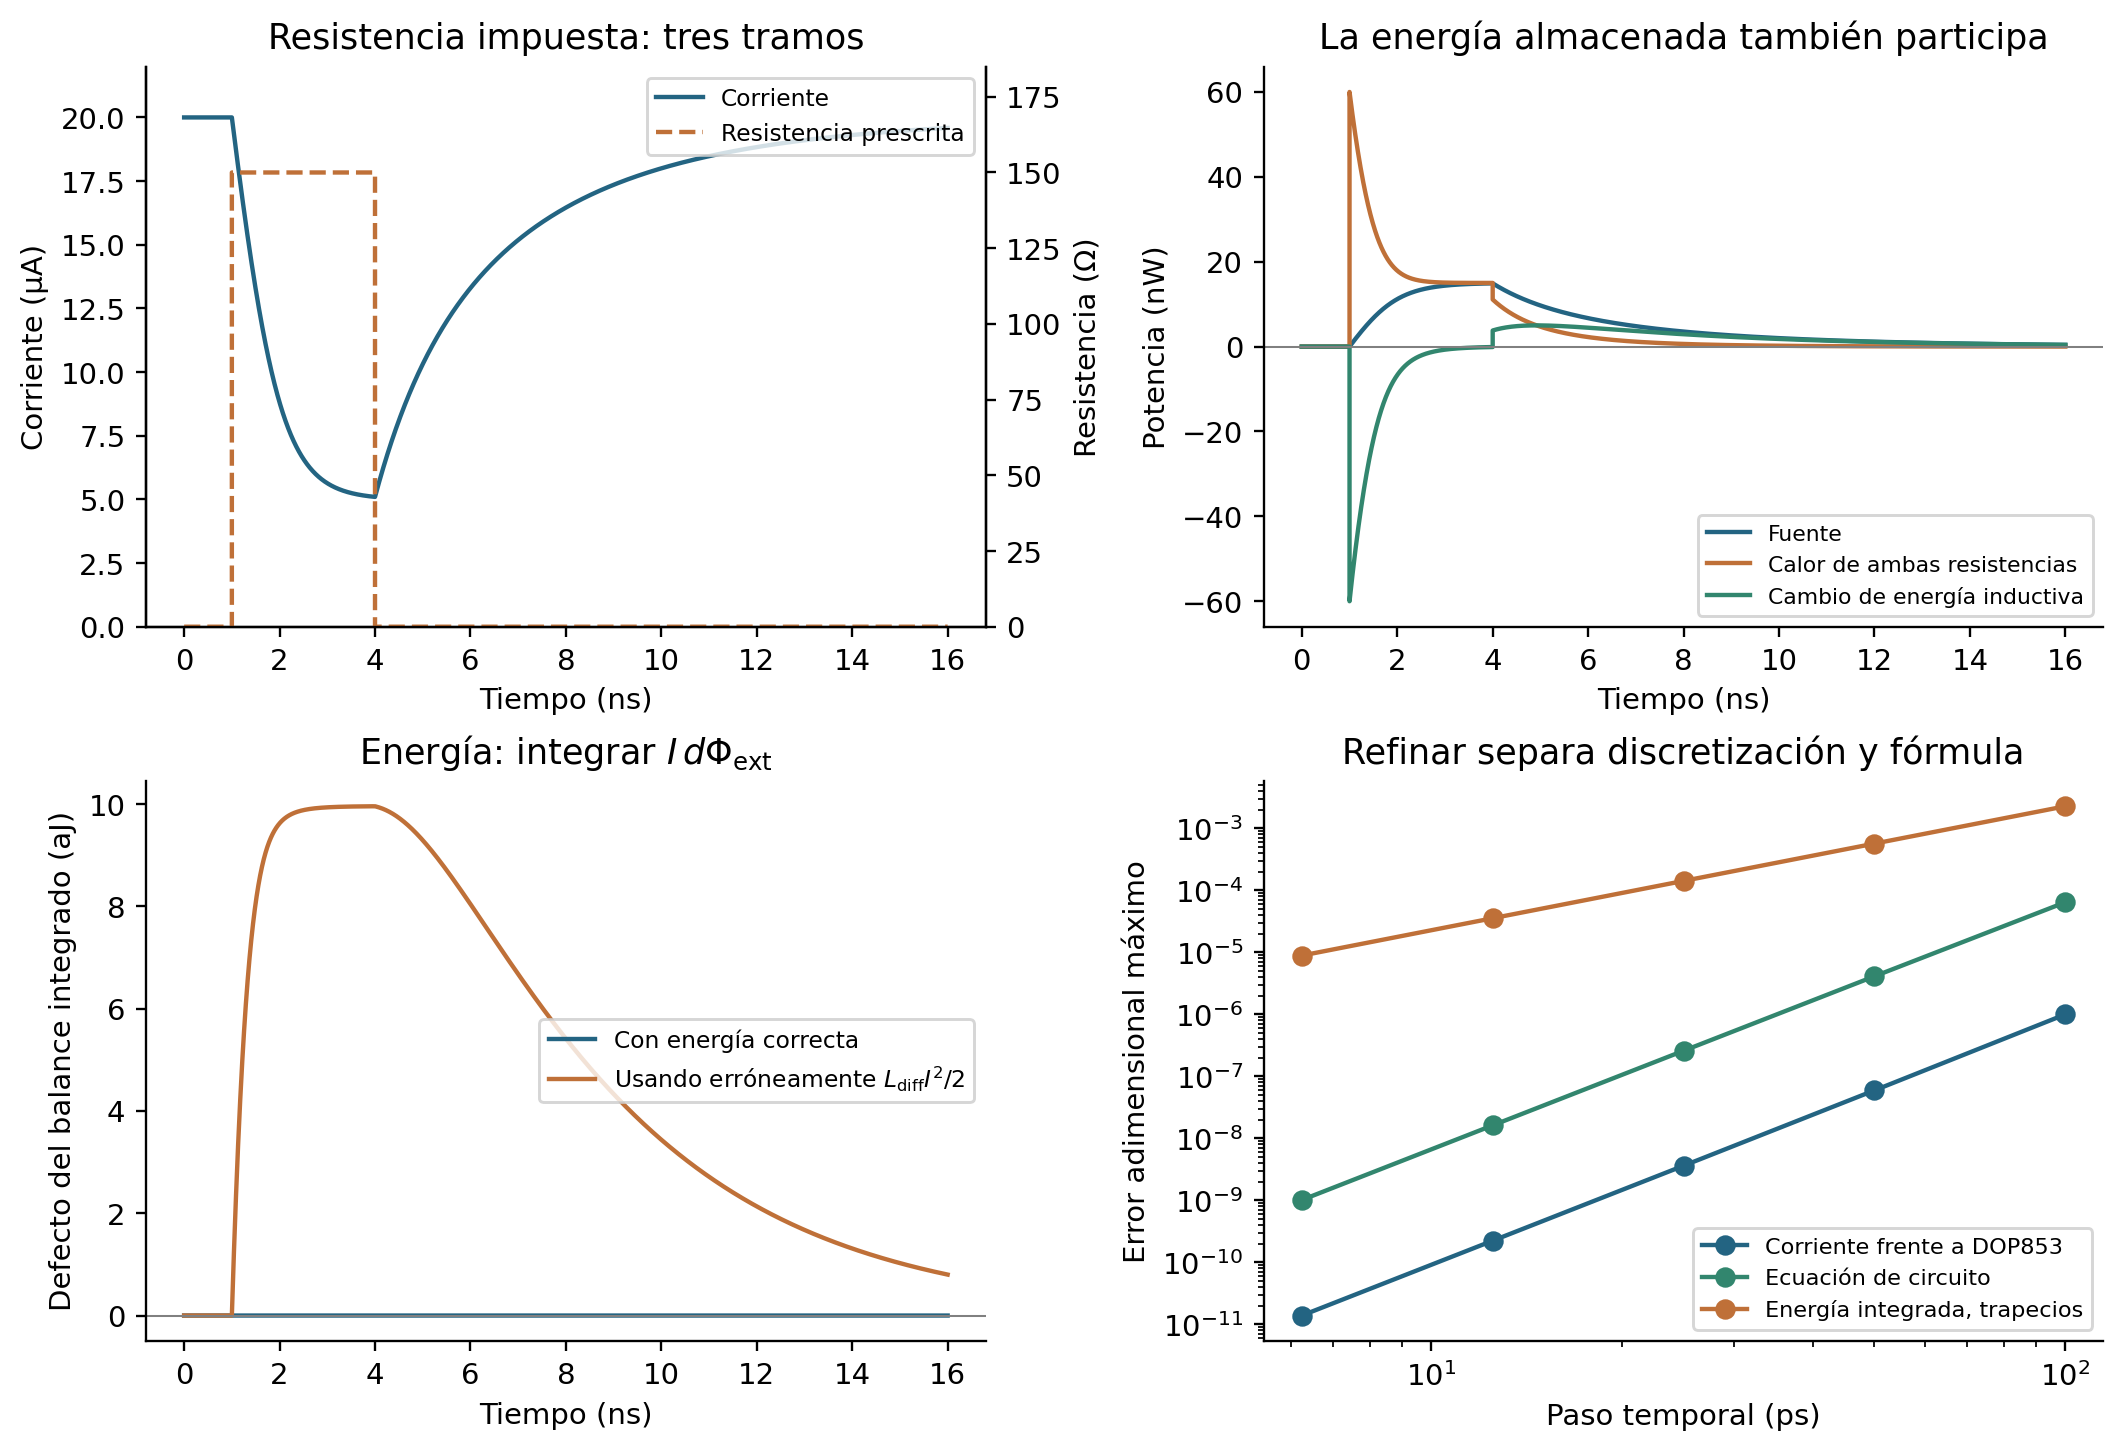
\includegraphics[width=0.98\linewidth,height=\textheight,keepaspectratio,alt={Figura D.1. Diagnóstico circuital independiente con resistencia prescrita. La redistribución de corriente genera el voltaje de puerto; la contabilidad incorpora la energía exterior derivada de la inductancia diferencial. Los parámetros son sintéticos y no representan una señal de detección calculada por A--C.}]{../figuras/D_01_circuito_y_balance.png}
\caption{Figura D.1. Diagnóstico circuital independiente con resistencia
prescrita. La redistribución de corriente genera el voltaje de puerto;
la contabilidad incorpora la energía exterior derivada de la inductancia
diferencial. Los parámetros son sintéticos y no representan una señal de
detección calculada por A--C.}
\end{figure}

Se usan \(I_b=20\,\mu\)A, \(R_L=50\,\Omega\), \(L_0=100\) nH y
\(\eta_L=1\). La resistencia prescrita es 0, 150 y 0 \(\Omega\) en los
intervalos 0--1, 1--4 y 4--16 ns. Cada tramo se integra por separado. Al
refinar el paso de 100 a 6.25 ps, la corriente y la ecuación circuital
muestran orden cuatro; la energía integrada por trapecios, orden dos. En
la malla fina, el error de corriente respecto de DOP853 es
\(1.38\times10^{-11}I_b\) y el defecto energético máximo es
\(3.55\times10^{-22}\) J. La fórmula incorrecta
\(L_{\rm ext}^{\rm diff}I^2/2\) deja un defecto \(9.96\times10^{-18}\)
J. El límite de inductancia constante coincide con la solución
exponencial a \(5.67\times10^{-11}I_b\).

Los parámetros, tolerancias, errores y datos completos se registran en
\nolinkurl{D04_circuito_y_balance.json} y dos CSV. Esta comprobación no
necesita un transitorio del detector para descubrir un error de energía
inductiva. Tampoco demuestra que la resistencia prescrita reproduzca un
dispositivo.

\subsection{D.3.2. Una condición espacial que la conservación no
garantiza}\label{d.3.2.-una-condiciuxf3n-espacial-que-la-conservaciuxf3n-no-garantiza}

El símbolo principal mide cómo responden las perturbaciones de longitud
de onda muy corta a las derivadas espaciales de mayor orden. Para
definirlo sin utilizar una fase singular, sea
\(z_1=\operatorname{Re}\Delta\), \(z_2=\operatorname{Im}\Delta\) y
\(\widehat{\mathbf k}\) una dirección espacial unitaria. La condición de
admisión del candidato es

\[
M_{ab}(\widehat{\mathbf k})=
\frac{\partial^2e_\delta}{\partial(\partial_i z_a)\partial(\partial_j z_b)}
\widehat k_i\widehat k_j,
\qquad \lambda_{\min}[M(\widehat{\mathbf k})]>0
\quad\text{para toda }\widehat{\mathbf k}.
\tag{D.36}
\]

Las derivadas mantienen fijos los campos locales y sus ocupaciones; se
suman \(i,j\). \(\lambda_{\min}\) es el menor valor propio de la matriz
real simétrica de dos componentes. Es una condición necesaria para
admitir el bloque del condensado, no una prueba completa del sistema
cinético acoplado. Con una movilidad positiva, un valor negativo permite
un crecimiento proporcional al cuadrado del número de onda. Reducir el
paso temporal no corrige ese defecto continuo. Un valor no positivo, o
una incertidumbre numérica que no permita certificar el signo, exige
detener y declarar no admisible la trayectoria; no se recorta la
rigidez.

La comprobación de C ofrece un contraejemplo explícito en una población
vacía: \(|\Delta|=0.60\Delta_0\), \(q\ell_0=1\) y
\(\delta=0.10\Delta_0\), donde \(\ell_0=\sqrt{\hbar D/(2k_BT_c)}\). La
rigidez de fase a amplitud fija es negativa, \(-0.34343\) en las
unidades declaradas en C. La contribución de Poisson es de orden
inferior en número de onda y no elimina este crecimiento. El resultado
es distinto de la pendiente de una rama cuya amplitud ya se minimizó:
aparece incluso fijando esa amplitud.

Esta condición restringe los ensayos posibles, pero no repara el modelo
en los estados rechazados. Un SNSPD puede explorar superflujo intenso y
amplitud reducida durante un evento; por ello no se asegura que una
trayectoria de detección permanezca dentro del dominio admitido. La
figura nueva de admisibilidad espacial de C y sus datos documentan el
diagnóstico. No se introduce una corrección de gradientes improvisada
para declarar resuelta esa dificultad.

\section{D.4. Secuencia de implementación y condiciones de
promoción}\label{d.4.-secuencia-de-implementaciuxf3n-y-condiciones-de-promociuxf3n}

El contrato continuo está fijado en D.1. La siguiente implementación
experimental debe discretizar esa misma energía y compartir cada flujo y
reacción entre sus balances. La secuencia reduce incertidumbres
distintas en cada paso:

\begin{enumerate}
\def\labelenumi{\arabic{enumi}.}
\tightlist
\item
  \textbf{Admitir datos y construir el catálogo.} Resolver las unidades
  fonónicas, los soportes y la normalización. Converger energía del
  vacío, derivadas y regulador espectral. Verificar que la tabla
  consultada en cada campo reproduce sus propias fuerzas y corriente.
\item
  \textbf{Acoplar una y dos celdas superconductoras.} Repetir con
  espectro móvil las pruebas que B realizó con DOS normal; incluir
  transporte entre gaps diferentes y remapeo a energía fija. Comprobar
  Pauli, positividad fonónica y energía sin recortes. Este punto todavía
  no está cubierto por la trayectoria normal de B ni por la celda sin
  transporte de C.
\item
  \textbf{Resolver el ensayo espacial admitido con bordes y circuito.}
  Comprobar primero D.36, sin proseguir una trayectoria que pierda esa
  propiedad. Comprobar flujos de interfaz, trabajo de reservorios y
  D.33; aumentar continuaciones hasta que la región central sea
  independiente de sus extremos. Converger espacio, tiempo y energías
  por separado, incluyendo sesgo de tabla. Mantener las mismas entradas
  materiales durante la comparación.
\item
  \textbf{Contrastar física del núcleo y de la disipación.} Medir
  sensibilidad de fuerzas, perfiles, barreras y primeros eventos de fase
  frente a una referencia espacial adecuada. El parámetro finito
  \(\delta=0.10\Delta_0\) no queda validado por tomar una malla más
  fina. Identificar \(\tau_{\rm kin}\) y contrastar movilidad KWT y
  reparto de calor en el régimen de uso.
\item
  \textbf{Comparar transitorios completos y promover sólo tras cumplir
  los criterios.} Comparar amplitud, distribuciones, corrientes, ambos
  voltajes, tiempos de primeros eventos de fase y balance, a iguales
  geometría, energía retenida y condiciones de borde. Separar el tiempo
  desde \(t_0\) de la etapa óptica omitida.
\end{enumerate}

Las tolerancias de aceptación se fijarán antes de comparar trazas, en
función de los observables requeridos y la precisión experimental. Las
pruebas presentes no permiten asignar honestamente una tolerancia
universal de latencia. Un residuo pequeño de energía es necesario, pero
no prueba la corrección del cierre ni la convergencia de un evento de
nucleación.

\textbf{Estado al cierre de 0.4:} catálogo y balances parciales
verificados; candidato continuo restringido documentado; pérdida de
positividad espacial detectada; datos fonónicos, núcleo y cinética
absoluta todavía no admitidos para predicción material. Se conserva
producción sin cambios. Los hallazgos indican exactamente qué verificar
antes de esperar un comportamiento fiable en transitorios completos.

\section{D.5. Archivos, reproducción y lectura del
cuaderno}\label{d.5.-archivos-reproducciuxf3n-y-lectura-del-cuaderno}

La entrega contiene cinco Markdown, cinco PDF, sus fuentes LaTeX,
figuras PNG/PDF, scripts de \nolinkurl{sandbox/model_v0_4} y resultados
de \nolinkurl{docs/modelo_v0_4/verificaciones}. Cada cálculo escribe
versiones de bibliotecas, residuos y datos; el manifiesto final enlaza
los archivos por SHA-256. La copia de Geminga se verifica contra esos
hashes. Los scripts de construcción documental no ejecutan el solver
físico.

El cuaderno vigente E-r02 tiene ocho clases activas y 24 respuestas
pendientes. La antigua clase de Nambu se retira y se reemplaza por
ocupaciones/operadores y luego una columna Nambu de dos modos.
Variaciones parte de una curva de perturbación; modos/DOS, DFT y DFPT se
desarrollan en clases separadas. E09 y E10 sustituyen la anterior E08.
La revisión del cuaderno se registra independientemente de la edición
física 0.4. No se supone aprobada ninguna clase por ausencia de
respuesta, ni se incluyen respuestas atribuidas al lector.

La procedencia técnica se mantiene cerca de cada bloque de D.1. Para las
derivaciones y fuentes primarias completas: A desarrolla el funcional
estático desde Virtanen et al.~y las convenciones de Usadel; B
desarrolla reacciones, energía adiabática y datos fonónicos con
Vodolazov, Allmaras y Simon et al.; C deriva la extensión espacial
efectiva, la ley compleja y el balance circuital. Los cierres efectivos
añadidos en esta iteración se identifican como tales y no se atribuyen a
una deducción microscópica que las referencias no proporcionan.

\end{document}
